\chapter{How to implement NIOS-designs}\label{NiosQuartusModelsim}
\chapterquote{The most important is, the Lord is one, and you shall love the Lord your God with all your heart and with all your soul and with all your mind and with all your strength. The second is this, you should love your neighbor as yourself.}{Jesus Christ}

\graphicspath{{BackMatters/Appendix/NiosOverview/}}
\lstinputpath{BackMatters/Appendix/NiosOverview/Codes} %path is defined in mypreamble

\textbf{Please implement the designs of Chapter \ref{ch:FirstProject} (i.e. Verilog design) and Chapter \ref{ch:NiosOverview} (i.e. NIOS design), before following this section.}

\begin{noNumBox}
	Note that, this appendix uses the VHDL file, but same procedure is applicable for Verilog projects as well. Codes files used in this section, are available in the folder `Appendix-How\_to\_implement\_Nios\_design', which can be \href{http://pythondsp.readthedocs.io/en/latest/pythondsp/toc.html}{downloaded from the website}. 
\end{noNumBox}

Unlike VHDL designs, NIOS designs can not be run directly on a system just by downloading it. Therefore, only required design-files are provided (instead of complete) for NIOS systems. We need to follow the steps provided in this section, to implement the NIOS design on the FPGA. 


Note that \textbf{VHDL codes} and \textbf{C/C++} codes of the tutorials are available on the website; these codes are provided inside the folders with name VHDLCodes (or vhdl) and CppCodes (or c, or software/ApplicationName\_app) respectively. Along with these codes, \textbf{.qsys files} are also provided, which are used to generated the .sopc and .sopcinfo files. Lastly, \textbf{pin assignments files} for various Altera-boards are also provided in the zip folders. 

\textbf{Please follow the below step, to compile the NIOS design on new system. Further, if you change the location of the project in the computer (after compiling it successfully), then NIOS design must be implemented again by following the instruction in Section \ref{sec:nios_again_implement}}



\section{Create project} \label{app:CreateProject}
First create a new Quartus project (with any name) as shown in Section \ref{sec:new_project}; and copy all the downloaded files (i.e. VHDLCodes, CppCodes, Pin-assignments  and .qsys files) inside the main project directory. 

\section{Add all files from VHDLCodes folder}

\begin{itemize}
	\item Next, add all the files inside the folder `VHDLCodes', to project as shown in Fig. \ref{fig:add_all_VHDLCodes}. \textbf{Do not forget to select `All files' option while adding the files as shown in Fig. \ref{fig:add_all_VHDLCodes}. } 
	
	\begin{figure}[!h]
		\centering
		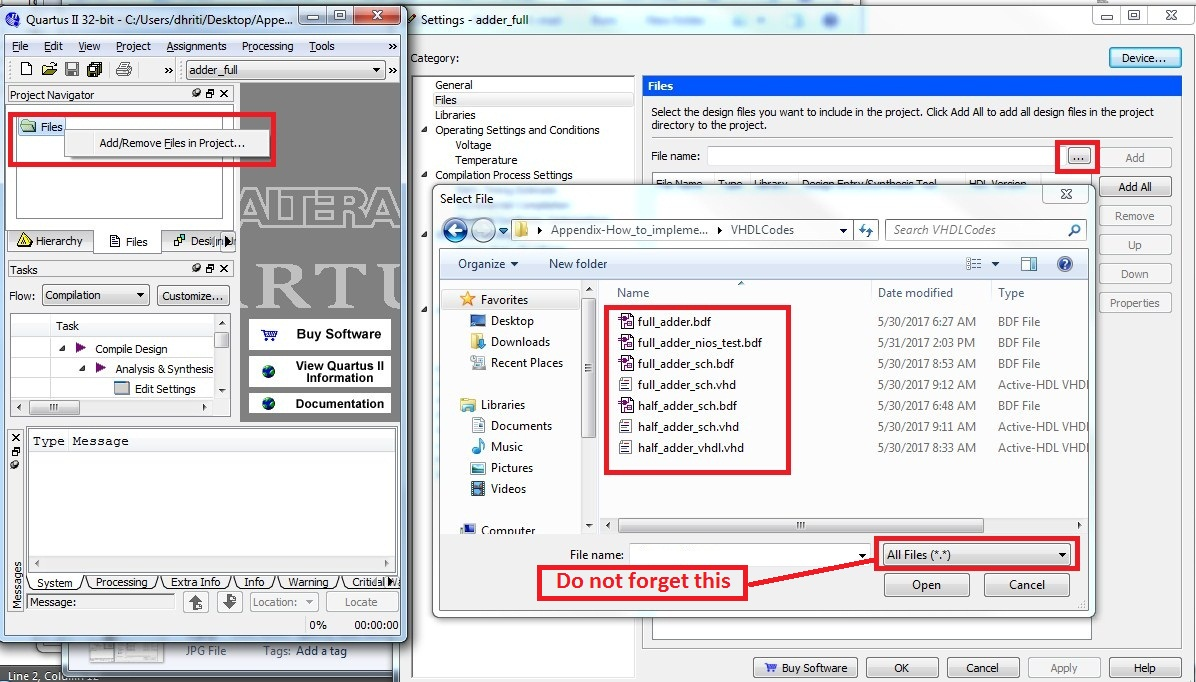
\includegraphics[width=\textwidth]{1}
		\caption{Add all files from VHDLCodes folder}
		\label{fig:add_all_VHDLCodes}
	\end{figure}
		
	\item In Chapter \ref{ch:FirstProject}, we created  `VHDLCodes' from the `Block schematic design'. These two designs are same, therefore while compilation the multiple-design error will be reported. Therefore we need to remove the duplicate designs as shown in Fig. \ref{fig:remove_duplicate}.  Note that, there are two duplicate designs i.e. one for half\_adder and other is for full\_adder as shown in the figure. 
	\begin{figure}[!h]
		\centering
		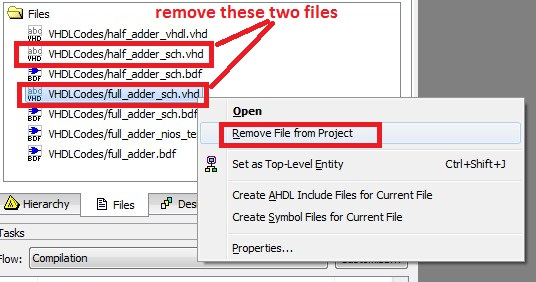
\includegraphics[scale=0.75]{2}
		\caption{Add all files from VHDLCodes folder}
		\label{fig:remove_duplicate}
	\end{figure}

	
	\item In this project, `full\_adder\_nios\_test.bdf' is the top-level design, which is shown in Fig. \ref{fig:full_adder_top_d}. Note that, here `name method' is used to connect the `addr\_input[2..0] with port `a', `b' and `c'. The method for giving name to a wire is shown in figure (see on the bottom-left side). 
	
	\begin{figure}[!h]
		\centering
		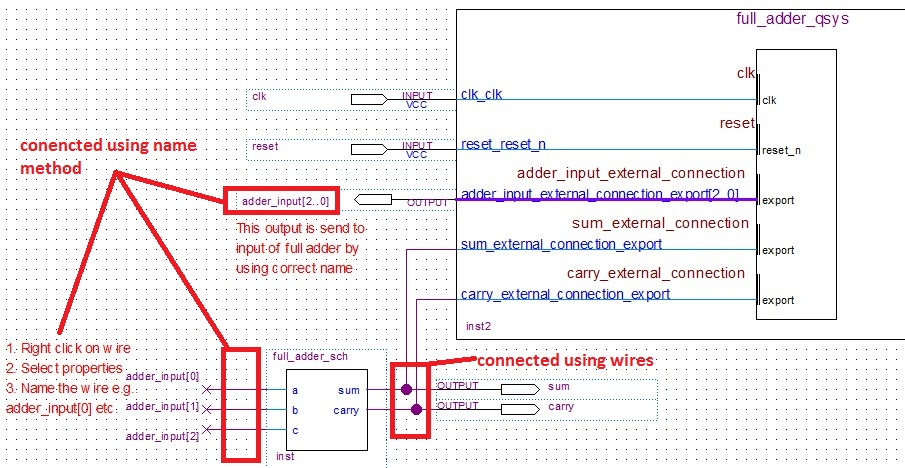
\includegraphics[scale=0.65]{4}
		\caption{Select this design i.e. `full\_adder\_nios\_test.bdf' as top level entity}
		\label{fig:full_adder_top_d}
	\end{figure}
	
	\item Now, select `full\_adder\_nios\_test.bdf' as the top level entity, as shown in Fig. \ref{fig:select_top_ent}.
	
	\item Modify the pin-assignment file and import it to the project . Also, make sure that correct FPGA-device is selected for the project. If problem in pin-assignments or device selection, then see Chapter \ref{ch:FirstProject} again. 
\end{itemize}


\section{Generate and Add QSys system}

Open the Qsys from Tools$\rightarrow$Qsys; and then open the downloaded `.qsys' file and follow the below steps, 

\begin{itemize}
	\item First, refresh the system, by clicking on Files$\rightarrow$Refresh System.
	
	\item Next, select the correct the device type as shown in Fig. \ref{fig:changeDevice}. 
	
	\item Now, assign base addresses and interrupt numbers by clicking on System$\rightarrow$`Assign base addresses' and `Assign interrupt numbers'.
	
	\item If there are some errors after following the above steps, then delete and add the Nios-processor again; and make the necessary connection again i.e. clock and reset etc. Sometimes we may need to create the whole Qsys-design again, if error is not removed by following the above steps. 
	
	\item Finally, generate the system as shown in Fig. \ref{fig:generate_system} ( or refer to  Fig. \ref{fig:simulationQsys} for generating system, if simulation is also used for NIOS design). Finally, close the Qsys after getting the message `Generate Completed'. 
	
	\item Finally, add the Qsys design to main project. For this, we need to add the `.qip' file generated by Qsys, which is available inside the synthesis folder. To add this file, follow the step in Fig \ref{fig:add_all_VHDLCodes}. You need to select the 	`All files' option again to see the `.qip file' as shown in Fig. \ref{fig:add_qsys_sys}. 
	
	
	\item Now, compile and load the design on FPGA system. 
\end{itemize}


\section{Nios system} \label{sec:nios_again_implement}

Next, we need to create the NIOS system. For this, follow the below steps, 
\begin{itemize}
	\item Follow the steps in Section \ref{sec:Nios_create_sys} and \ref{sec:add_modify_bsp} to create the NIOS-BSP file. Note that, you need to select the `.sopcinfo' file, which is inside the current main-project-directory.  

	\item Next, we need to create the application file. To create the application, go to File$\rightarrow$New$\rightarrow$Nios II Application. Fill the application name e.g. `Application\_fullAdder' and select the BSP location as shown in Fig. \ref{fig:createApplication}. \textbf{Note that, if `c code' is provided inside the `software folder (not in the `CppCodes' or `c' folders)' e.g. `software/fullAdder\_app', then copy and paste folder-name as the application name i.e. `fullAdder\_app' to create the application file. Note that, we usually add `\_app' at the end of application name and `\_bsp' at the end of BSP name. In this case, `c code' will automatically added to the project. Next, right click on the `c file' and select `add to NIOS II build'; and skip the next step of adding `c file', as it is already added in this case. Please see the ``video \href{https://www.youtube.com/playlist?list=PLpqu8JfoNKiNJpFvKTeBlI-LMzc2TAlRM}{Appendix - How to implement NIOS design }'', if you have problem in this part of tutorial.}
	
%	\item Next, import the `c/c++' file from the CppCodes folder. For this, right click on the application i.e. `Application\_fullAdder' and click on the `import'. Then click on `General' and select `File System' 

	\item Next, we need to import the `c' code from folder `CppCodes (or c)'. For this, right click on the application and click on Import$\rightarrow$General$\rightarrow$File System$\rightarrow$From Directory; browse the directory, where we have saved  the CppCodes  and select the files as shown in Fig. \ref{fig:AddCfiles}. Finally, simulate the system as described in Section \ref{sec:SimulateNios}.
	
	\item Finally, simulate or load the design on FPGA. Please refer to Section \ref{sec:SimulateNios} for simulation; and to Section \ref{sec:AddLoadNIOS} for loading the NIOS design on FPGA. \textbf{Do not forget to keep reset button high, while loading the NIOS II design.} 
	
	\item The current example will display the outputs on NIOS terminal, as shown in Fig. \ref{fig:Final_adder_out}. Also, sum and carry values will be displayed on the LEDs.  
	
	
\end{itemize}

\begin{figure}[!h]
	\centering
	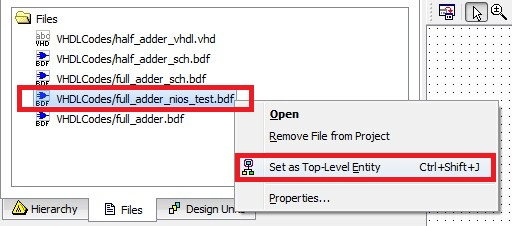
\includegraphics[scale=0.8]{3}
	\caption{Select top level entity}
	\label{fig:select_top_ent}
\end{figure}

\begin{figure}[!h]
	\centering
	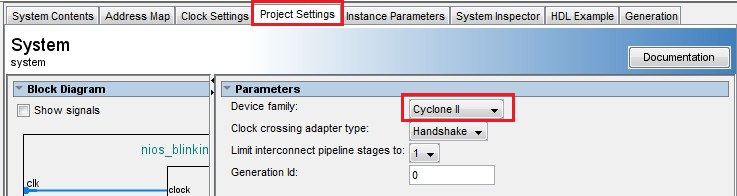
\includegraphics[scale=0.7]{changeDevice}
	\caption{Change device family}
	\label{fig:changeDevice}
\end{figure}

\begin{figure}[!h]
	\centering
	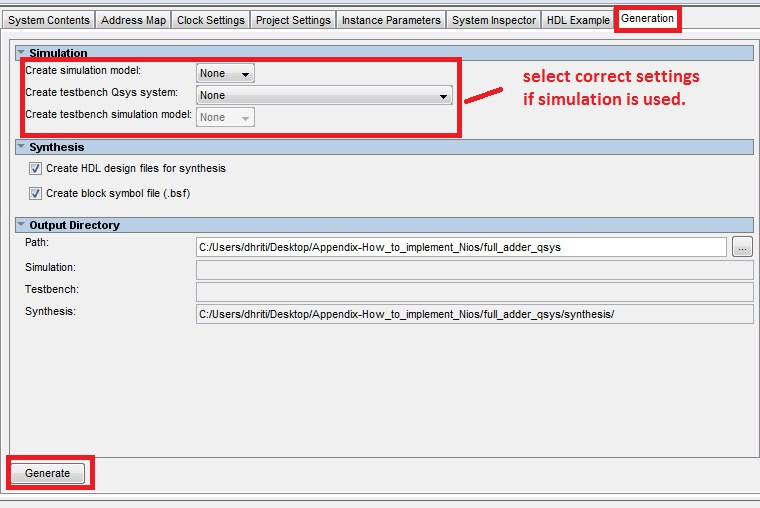
\includegraphics[scale=0.7]{5}
	\caption{Generate QSys system}
	\label{fig:generate_system}
\end{figure}

\begin{figure}[!h]
	\centering
	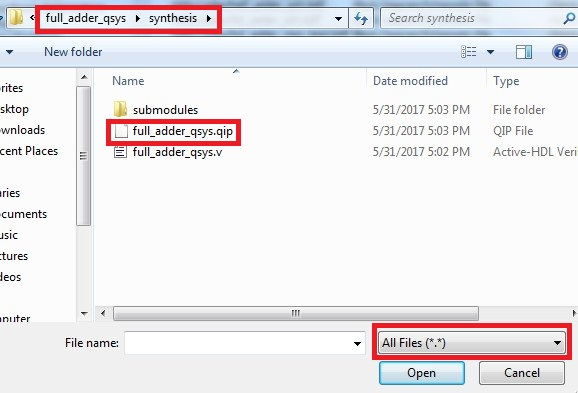
\includegraphics[scale=0.65]{6}
	\caption{Change device family}
	\label{fig:add_qsys_sys}
\end{figure}

\begin{figure}[!h]
	\centering
	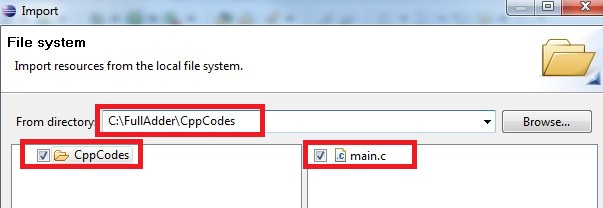
\includegraphics[scale=0.65]{AddCfiles}
	\caption{Adding C files}
	\label{fig:AddCfiles}
\end{figure}

\begin{figure}[!h]
	\centering
	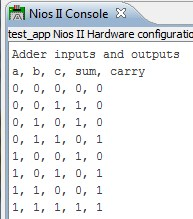
\includegraphics[scale=0.8]{7}
	\caption{Nios Output of current design}
	\label{fig:Final_adder_out}
\end{figure}


%%%%%%%%%%%%%%%%%%%%%%%%%%%%%%%%%%%%%%%%%%%%%%%%%%%% old %%%%%%%%%%%%%%%%%%%%%%%%%%%%%%%%%%%%%%%%%%%

%
%\section{Generate Qsys system}
%This section is required, if the provided codes on the website contain the `.qsys' file, otherwise jump to section \ref{sec:topLevelEntity}. 
%
%Open the Qsys from Tools$\rightarrow$Qsys; and then open the downloaded `.qsys' file. Now, we need to change the device type, if the board is not from `cyclone-II' family. For this, go to `Project settings' and select the correct device family as shown in Fig. \ref{fig:changeDevice}. Finally, generate the system according to Fig. \ref{fig:simulationQsys}. 
%
%\begin{figure}
%	\centering
%	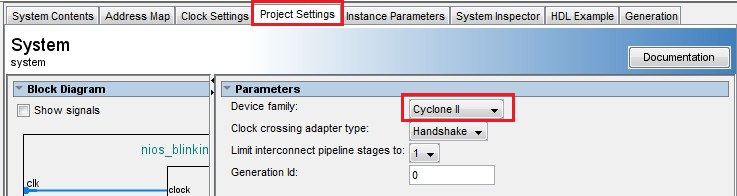
\includegraphics[scale=0.6]{changeDevice}
%	\caption{Change device family}
%	\label{fig:changeDevice}
%\end{figure}
%
%\begin{noNumBox}
%	Also, This step (i.e. creating NIOS processor) is mandatory for the cases, where the Family of FPGA board is changed i.e. Cyclone-IV is used instead of Cyclone-II.
%\end{noNumBox}
%
%\section{Nios processor} \label{sec:Nios_processor_location}
%Now, create the NIOS processor by following the steps in Sections  \ref{sec:AddBSP} and  \ref{sec:ModifyBSP}. Then, add the application as discussed in section \ref{sec:AddApplication}. Next, to add the `C/C++' files in the application, right click on the application and click on Import$\rightarrow$General$\rightarrow$File System$\rightarrow$From Directory; browse the director, where you have downloaded the codes and select the files as shown in Fig. \ref{fig:AddCfiles}. Finally, simulate the system as described in Section \ref{sec:SimulateNios}.
%
%\begin{figure}
%	\centering
%	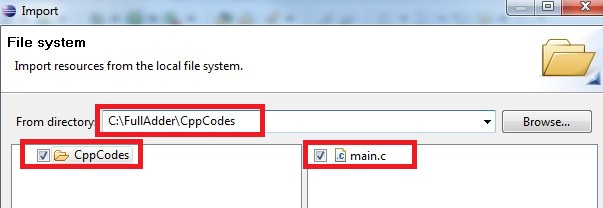
\includegraphics[scale=0.6]{AddCfiles}
%	\caption{Adding C files}
%	\label{fig:AddCfiles}
%\end{figure}
%
%\begin{noNumBox}
%	Also, This step (i.e. creating NIOS processor) is mandatory for the cases, where the location of the project is changed in the computer or the FPGA board is changed.
%\end{noNumBox}
%
%\section{Adding VHDL files} \label{sec:topLevelEntity}
%All the VHDL files are provided on the website and `.qip' files are generated by steps described in Section \ref{app:CreateProject}. To add the .qip file, right-click on the files and then click on the add-and-remove-files-in the project and locate the .qip file in the synthesis folder as shown in Fig. \ref{fig:AddQip}. 
%
%Also, VHDLCodes (or vhdl) folder may contain various types of files (depending on the design) e.g. `.vhd', `.qip' and `.bsf' etc. \textbf{We need to add add these files to the project.} To add these files, we need to choose the option `All Files' as shown in Fig. \ref{fig:addAllFiles} and then select all the files. 
%
%\begin{figure}
%	\centering
%	\includegraphics[scale=0.65]{addAllFiles}
%	\caption{Adding all files from VHDLCodes (or vhdl) folder}
%	\label{fig:addAllFiles}
%\end{figure}
%
%\section {Load the VHDL design on FPGA}
%
%Next, go to the files and right-click on the vhdl file to which you want to execute and click on `Set as Top-Level Entity' as shown in Fig. \ref{fig:Quartus}; and compile and load the design (if problem in loading the design, then see Appendix \ref{QuartusModelsim}.)
%
%
%\section{Load the Nios design on FPGA}
%Finally, follow the steps in Section \ref{sec:AddLoadVHDL} and \ref{sec:AddLoadNIOS} to load the designs on FPGA i.e. `.sof' file and `.elf' files respectively. 
%%%%%%%%%%%%%%%%%%%%%%%%%%%%%%%%%%%%%%%%%%%%%%%%%%%% old %%%%%%%%%%%%%%%%%%%%%%%%%%%%%%%%%%%%%%%%%%%